\documentclass[titlepage,a4paper]{article}

\usepackage{a4wide}
\usepackage[colorlinks=true,linkcolor=black,urlcolor=blue,bookmarksopen=true]{hyperref}
\usepackage{bookmark}
\usepackage{fancyhdr}
\usepackage[spanish]{babel}
\usepackage[utf8]{inputenc}
\usepackage[T1]{fontenc}
\usepackage{graphicx}
\usepackage{float}

\pagestyle{fancy} % Encabezado y pie de página
\fancyhf{}
\fancyhead[L]{TP2 - G15}
\fancyhead[R]{Algoritmos y Programación III - FIUBA}
\renewcommand{\headrulewidth}{0.4pt}
\fancyfoot[C]{\thepage}
\renewcommand{\footrulewidth}{0.4pt}

\begin{document}
\begin{titlepage} % Carátula
	\hfill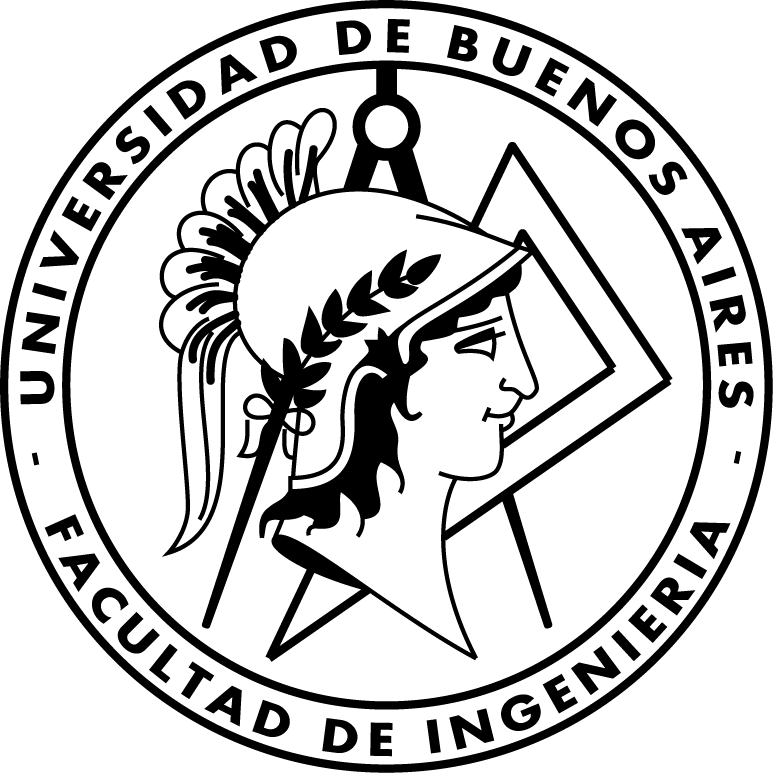
\includegraphics[width=6cm]{logofiuba.jpg}
    \centering
    \vfill
    \Huge \textbf{Trabajo Práctico 2 — Java}
    \vskip2cm
    \Large [7507/9502] Algoritmos y Programación III\\
    Grupo G15 \\
    Primer cuatrimestre 2022 \\
    \vfill
    Integrantes \\
    .\\
    \begin{tabular}{ | l | l | l | } % Datos del alumno
      \hline
      Alumno & Padrón & Email \\ \hline
      Alvaro Martin & 105040 & alvaro.martin1307@gmail.com \\ \hline
      Integrante2 & padron2 & email2 \\ \hline
      Integrante3 & padron3 & email3 \\ \hline
      Integrante4 & padron4 & email4 \\ \hline
      Integrante5 & padron5 & email5 \\ \hline
  	\end{tabular}
    \vfill
    \vfill
\end{titlepage}

\tableofcontents % Índice general
\newpage

\section{Introducción}\label{sec:intro}

\section{Supuestos}\label{sec:supuestos}
% Deberá contener explicaciones de cada uno de los supuestos que el alumno haya tenido que adoptar a partir de situaciones que no estén contempladas en la especificación.

\section{Diagramas de clase}\label{sec:diagramasdeclase}
% Uno o varios diagramas de clases mostrando las relaciones estáticas entre las clases.  Puede agregarse todo el texto necesario para aclarar y explicar su diseño. Recuerden que la idea de todo el documento es que quede documentado y entendible cómo está implementada la solución.

\begin{figure}[H]
\centering
% \includegraphics[width=0.8\textwidth]{diagrama_clase01.png}
\caption{\label{fig:class01}Explicacion diagrama}
\end{figure}

\section{Detalles de implementación}\label{sec:implementacion}

Explicación del modelo inicial

\subsection{Primer entrega}

\subsubsection[]{Una moto atraviesa la ciudad y se encuentra con un Pozo. Es penalizada en tres movimientos}

Info sobre 4.1.1

\subsubsection[]{Un auto atraviesa la ciudad y se encuentra con un Pozo. Es penalizada en tres movimientos}

Info sobre 4.1.2

\subsubsection[]{Una 4x4 atraviesa la ciudad y se encuentra con un Pozo. No es penalizada}

Info sobre 4.1.3

\section{Excepciones}\label{sec:excepciones}
% Explicación de cada una de las excepciones creadas y con qué fin fueron creadas.

\begin{description}
\item[Exception] Explicacion excepcion 1
\item[Excepcion] Explicacion excepcion 2
\end{description}

\section{Diagramas de secuencia}\label{sec:diagramasdesecuencia}
% Mostrar las secuencias interesantes que hayan implementado. Pueden agregar texto para explicar si algo no queda claro.

Introducción

\begin{figure}[H]
\centering
% \includegraphics[width=0.8\textwidth]{diagrama_secuencia01.png}
\caption{\label{fig:seq01}Titulo de secuencia}
\end{figure}

Breve explicacion secuencia 

\begin{figure}[H]
\centering
% \includegraphics[width=\textwidth]{diagrama_secuencia02.png}
\caption{\label{fig:seq02}Titulo de secuencia}
\end{figure}

Breve explicacion secuencia

\end{document}